
\documentclass[conference,compsoc,onecolumn]{IEEEtran}

\usepackage[utf8]{inputenc}
\usepackage[spanish]{babel}
\usepackage{amsmath}
\usepackage{graphicx}
\usepackage{subcaption}
\usepackage{amsfonts}
\usepackage{amssymb}
\usepackage{wrapfig}
\usepackage{float}

\title{Proyecto de curso}
\author{\IEEEauthorblockN{Dennis Adriana González Cifuentes}
\IEEEauthorblockA{\textit{Ciencias Naturales e Ingeniería\\Universidad Jorge Tadeo Lozano\\Bogotá - Colombia\\dennisa.gonzalezc@utadeo.edu.co} 
}
\and
\IEEEauthorblockN{María Fernanda López Martínez}
\IEEEauthorblockA{\textit{Ciencias Naturales e Ingeniería\\Universidad Jorge Tadeo Lozano\\Bogotá - Colombia\\mariafe.lopezm@utadeo.edu.co}}
\and
}
\graphicspath{{Imagenes/}}

\renewcommand\IEEEkeywordsname{Palabras cláve}

\begin{document}
    \maketitle
    \begin{abstract} 
        En el presente documento se encuentra el proyecto  de Inteligencia Artificial, en el cual se presentará la extracción, pre-procesamiento, visualización y análisis de los datos escogidos previamente \textit{(Notas obtenidas por estudiantes en varias asignaturas)}, el cual se realizará por medio de la metodología y las herramientas presentadas en el curso.\\
       
    \end{abstract}
    
    \begin{IEEEkeywords}
        Notas, asignaturas, calificaciones, estudiantes, Estados Unidos, grupos étnicos, matemáticas, lectura, escritura.
    \end{IEEEkeywords}

\section{Marco teórico}\label{marcoTeorico}
    La recolección de notas obtenidas de estudiantes de secundaria en un colegio ubicado en Estados Unidos, nos brindan todo tipo de información la cual será realizada e intrepretada en el presente documento, con el fin de encontrar y visualizar las principales características estadísticas de estos utilizando las herramientas vistas en
    clases\\
    
\section{Visualización}\label{resultados}
   Para empezar se deben importar las librerías adecuadas para la realización del trabajo, el cual se escogío un conjunto de datos de las \textit{Notas obtenidas por estudiantes en varias asignaturas de secuandaria} 
    \begin{figure}[H]
     \centering
            {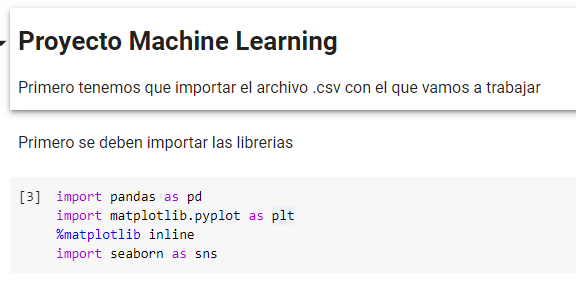
\includegraphics[scale = 0.90]{librerias.PNG}}
            \caption{Importación de librerías}
            \label{subfigura1}
    \end{figure}
    
    \begin{figure}[H]
            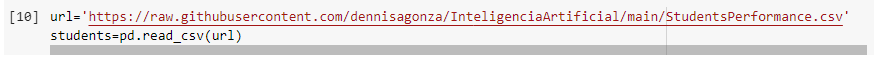
\includegraphics[scale=0.80]{datos.png}
            \caption{Importación del archivo}
            \label{subfigura2}
            \vspace{0,5cm}
    \end{figure}
    \begin{figure}[H]       
            \centering
            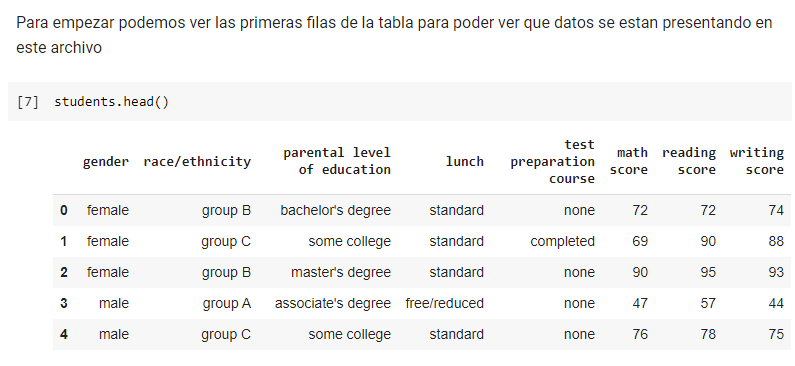
\includegraphics[scale = 0.80]{head.png}
            \caption{Visualización de las primeras filas de la tabla}
            \label{subfigura3}
             \vspace{0,5cm}
       
    \end{figure}
    
    A partir de la gráfica anterior, filtramos los tres mejores puntajes los cuales podemos observar que dos son femeninos y uno masculino, los cuales pertenecen al grupo étnico E, las tres personas sacaron en todas las materias un puntaje máximo de 100 y solo el hombre realizo un curso de preparación para el mismo.
    
    \begin{figure}[H]
            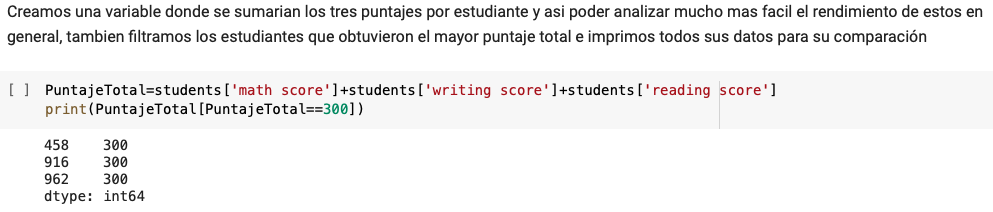
\includegraphics[scale = 0.50]{1.png}
            \caption{Visualización de datos filtrados para su correcta comparación y análisis}
            \label{subfigura4}
             \vspace{0,5cm}
       
    \end{figure} 
    \begin{figure}[H]
            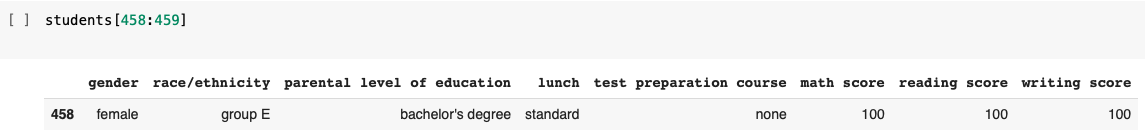
\includegraphics[scale = 0.50]{2.png}
            \caption{Visualización de datos filtrados}
            \label{subfigura18}
             \vspace{0,5cm}
    \end{figure} 
        
    \begin{figure}[H]       
        \centering
        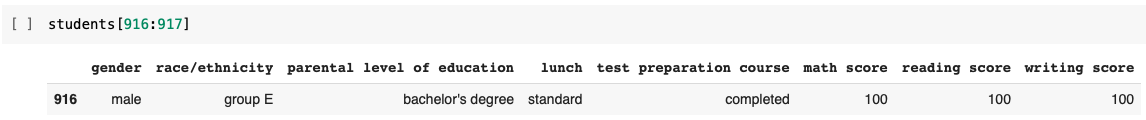
\includegraphics[scale = 0.4]{3.png}
        \caption{Visualización de datos filtrados}
        \label{subfigura16}
    \end{figure}
        
   
    \begin{figure}[H]       
        \centering
        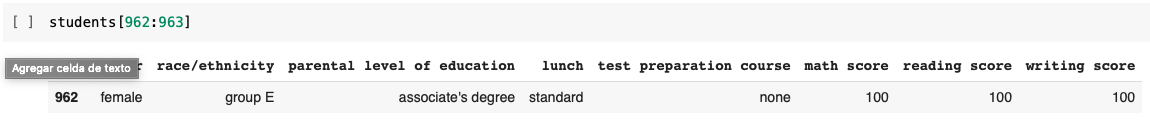
\includegraphics[scale = 0.48]{4.png}
        \caption{Visualización de datos filtrados}
        \label{subfigura10}
    \end{figure}
    
    A continuación, podremos observar en las siguientes gráficas la descripción de cada información de la columna de \textit{Puntajes}.
    
    En los cuales se puede observar que en todas las materias se obtuvo una calificación de 100 como puntaje máximo, mientras que la media varia entre 66 a 69. Y, como puntaje mínimo se obtiene una variación de las calificaciónes entre 0 a 17, el cual matemáticas obtuvo el menor puntaje.
    
    
    El promedio de las calificaciones de los examenes en la materia de matemáticas es de 66, en el cual la calificación mínima de 17 y la máxima es de 100.
    
     \begin{figure}[H]       
            \centering
            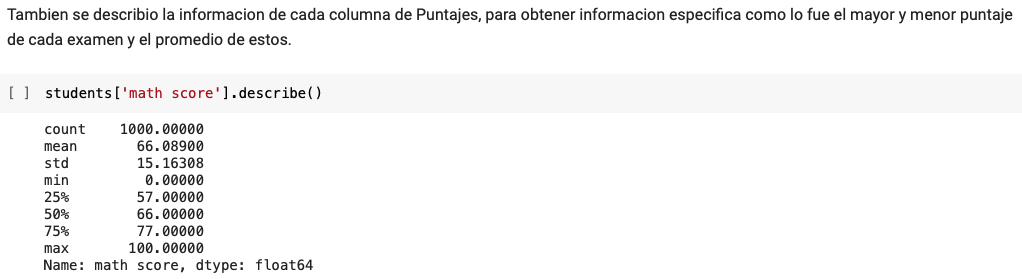
\includegraphics[scale = 0.50]{5.png}
            \caption{Descripción de la información de datos de los puntajes del área de matemáticas}
            \label{subfigura8}
        \end{figure}
    El promedio de las calificaciones de los examenes en la materia de lectura es de 69, en el cual la calificación mínima de 17 y la máxima es de 100
         \begin{figure}[H]       
            \centering
            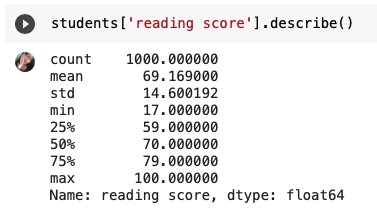
\includegraphics[scale = 0.50]{6.png}
            \caption{Descripción de la información de datos de los puntajes del área de lectura}
            \label{subfigura11}
        \end{figure}
    El promedio de las calificaciones de los examenes en la materia de escritura es de 68, en el cual la calificación mínima es de 10 y la máxima es de 100
         \begin{figure}[H]       
            \centering
            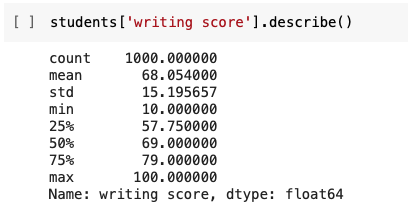
\includegraphics[scale = 0.50]{8.png}
            \caption{Descripción de la información de datos de los puntajes del área de escritura}
            \label{subfigura12}
        \end{figure}
        En esta gráfica se puede interpretar que el genero femenino obtuvo un mejor puntaje en todas las materias que el genero masculino.
         \begin{figure}[H]       
            \centering
            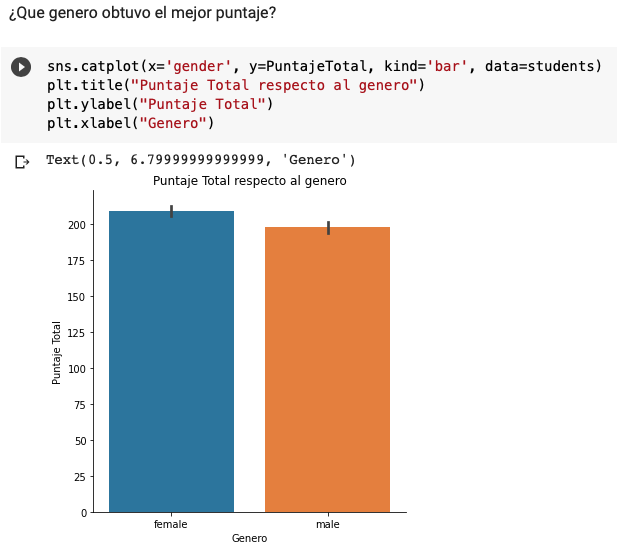
\includegraphics[scale = 0.50]{9.png}
            \caption{Gráfica de puntaje en el examen respecto a cada genero}
            \label{subfigura13}
        \end{figure}
        
        \par Para la siguiente gráfica se tomo el puntaje de cada examen respecto a si habian completado el test de preparación del curso. Como se puede evidenciar, si realizan un test de preparación no significa que van obtener los mejores puntajes, pero si se evidencia algún conocimiento previo puesto que no tienen tan bajos puntajes respecto a las personas que no realizaron el test.
        
        Por otro lado, se demuestra que evidentemente son muchos más estudiantes que obtuvieron los mejores puntajes si realizaron un test de preparación anteriormente, en cambio las personas que no lo realizaron estan sobre la media total de los puntajes.
         \begin{figure}[H]       
            \centering
            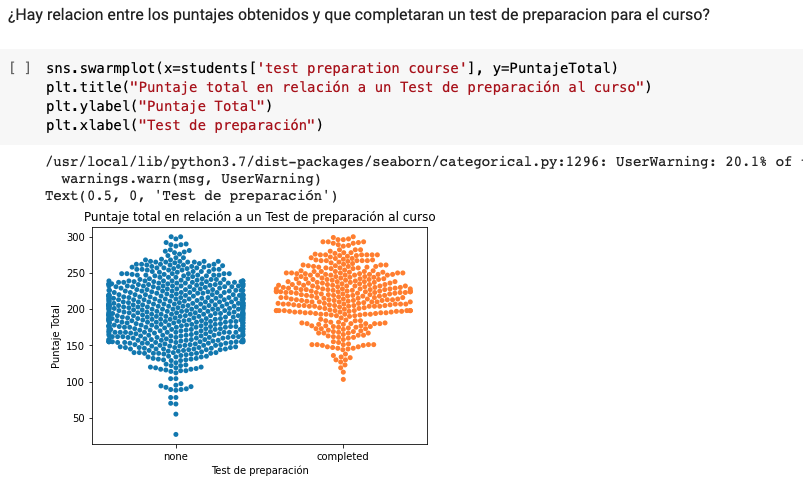
\includegraphics[scale = 0.50]{10.png}
            \caption{Gráfica de puntaje en el examen respecto a el examen de preparación del curso}
            \label{subfigura14}
        \end{figure}
        
         En la siguiente gráfica se puede visualizar que grupos étnicos tuvieron un mejor puntaje en todas las áreas de aprendizaje, como: matemáticas, lectura y escritura. En las cuales, podemos concluir que el grupo étnico E sobresale en las tres materias con puntajes altos, mientras que el grupo étnico A tiene los menores puntajes en todas las materias.
         \begin{figure}[H]       
            \centering
            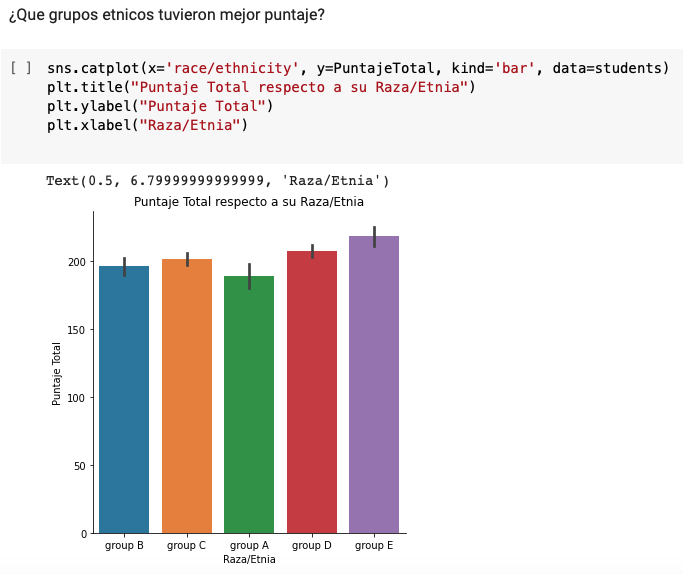
\includegraphics[scale = 0.50]{11.png}
            \caption{Gráfica de puntaje en cada grupo étnico}
            \label{subfigura15}
        \end{figure}
        
        \section{Conclusiones}\label{conclusiones}
        \begin{itemize}
        \item Al filtrar por los tres mejores puntajes de todos los estudiantes, se encontró a dos mujeres y dos hombres. Los cuales pertenecen al grupo étnico E, y solo el hombre realizó el curso de preparación para el ingreso al mismo.
        \item Los tres mejores estudiantes, obtuvieron en todas las asignaturas un puntaje máximo de 100 puntos.
        \item En las tres materias se obtuvo un puntaje máximo de 100 puntos, mientras que el puntaje mínimo se encuentra en en un rango de 0 a 17 puntos.
        \item En relación con todos los puntajes filtrado por generos, se encontró que el genero femenino tuvo un mayor puntaje en todas las materias que el genero masculino.
        \item El test de preparación se realiza para obtener conocimientos previos de las materias y no garantiza que saquen los mayores puntajes.
        \item Los puntajes filtrados por cada grupo étnico demuestran que el grupo E tiene los mayores puntajes, mientras que el grupo A los menores.
        \end{itemize} 
        
    \begin{thebibliography}{00}
    \bibitem{b1} J.Seshapanpu ``Students Performance in Exams'' Kaggle, url: https://www.kaggle.com/spscientist/students-performance-in-exams, Noviembre 2018.
    \bibitem{b2} Repositorio en Git https://github.com/dennisagonza/InteligenciaArtificial
    \end{thebibliography}
\end{document}
